% Slide 10 -- Feature 2: per-slice circles (consolidated)
\begin{frame}{Feature 2: per-slice articular circles}
  \begin{columns}[T]
    \begin{column}{0.5\textwidth}
      \begin{block}{Key idea}
        On equatorial slices, the articular contour is locally circular. Each fitted circle is an \alert{arc that lies on the cartilage} --- not an approximation of it.
      \end{block}
      \begin{block}{Clinical meaning}
        \begin{itemize}
          \item A focal \alert{drop in inlier ratio} signals loss of articular continuity --- a potential tear.
          \item Each circle is rendered as a PNG so the radiologist can \alert{verify it slice by slice}.
        \end{itemize}
      \end{block}
    \end{column}
    \begin{column}{0.5\textwidth}
      \centering
      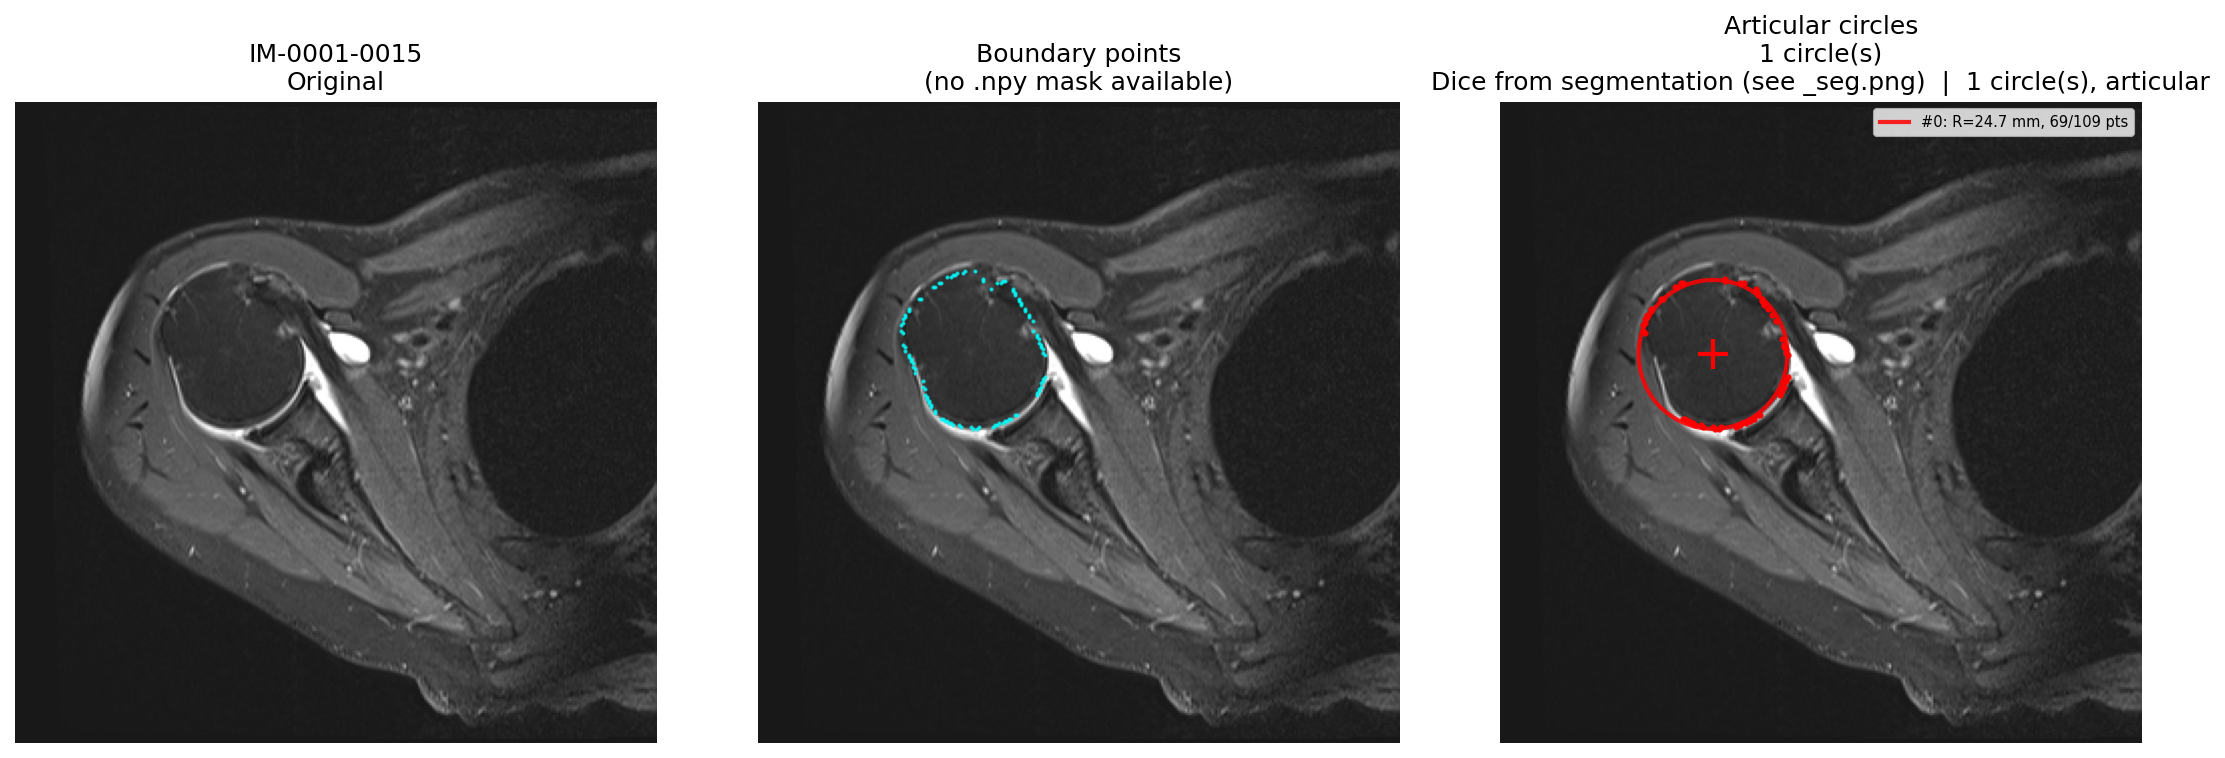
\includegraphics[width=\linewidth,height=0.7\textheight,keepaspectratio]{figures/circle_articular.png}
      \\[0.3em]
      {\scriptsize Image $\rightarrow$ mask $\rightarrow$ contour $\rightarrow$ fitted circle.}
    \end{column}
  \end{columns}
\end{frame}
